%package list
\documentclass{article}
\usepackage{amsmath}
\usepackage[top=3cm, bottom=3cm, outer=3cm, inner=3cm]{geometry}
\usepackage{multicol}
\usepackage{graphicx}
\usepackage{url}
%\usepackage{cite}
\usepackage{hyperref}
\usepackage{array}
%\usepackage{multicol}
\newcolumntype{x}[1]{>{\centering\arraybackslash\hspace{0pt}}p{#1}}
\usepackage{natbib}
\usepackage{pdfpages}
\usepackage{multirow}
\usepackage[normalem]{ulem}
\useunder{\uline}{\ul}{}
\usepackage{svg}
\usepackage{xcolor}
\usepackage{minted}

%\usepackage{booktabs}
\usepackage{caption}
\usepackage{subcaption}
\usepackage{float}
\usepackage{array}

\newcolumntype{M}[1]{>{\centering\arraybackslash}m{#1}}
\newcolumntype{N}{@{}m{0pt}@{}}

%%%%%%%%%%%%%%%%%%%%%%%%%%%%%%%%%%%%%%%%%%%%%%%%%%%%%%%%%%%%%%%%%%%%%%%%%%%%
%%%%%%%%%%%%%%%%%%%%%%%%%%%%%%%%%%%%%%%%%%%%%%%%%%%%%%%%%%%%%%%%%%%%%%%%%%%%
\newcommand{\itemEmail}{ccapatinta@unsa.edu.pe}
\newcommand{\itemStudent}{Capatinta Almanza Camilo B. A.}
\newcommand{\itemCourse}{Lab. Análisis y Diseño de Algoritmos}
\newcommand{\itemCourseCode}{1702231}
\newcommand{\itemSemester}{IV}
\newcommand{\itemUniversity}{Universidad Nacional de San Agustín de Arequipa}
\newcommand{\itemFaculty}{Facultad de Ingeniería de Producción y Servicios}
\newcommand{\itemDepartment}{Departamento Académico de Ingeniería de Sistemas e Informática}
\newcommand{\itemSchool}{Escuela Profesional de Ingeniería de Sistemas}
\newcommand{\itemAcademic}{2026 - B}
\newcommand{\itemInput}{05/11/2026}
\newcommand{\itemOutput}{--/11/2026}
\newcommand{\itemPracticeNumber}{08}
\newcommand{\itemTheme}{Métodos Heurísticos: Problemas NP y Búsqueda Aleatoria (Monte Carlo)}
%%%%%%%%%%%%%%%%%%%%%%%%%%%%%%%%%%%%%%%%%%%%%%%%%%%%%%%%%%%%%%%%%%%%%%%%%%%%
%%%%%%%%%%%%%%%%%%%%%%%%%%%%%%%%%%%%%%%%%%%%%%%%%%%%%%%%%%%%%%%%%%%%%%%%%%%%

\usepackage[english,spanish]{babel}
\usepackage[utf8]{inputenc}
\AtBeginDocument{\selectlanguage{spanish}}
\renewcommand{\figurename}{Figura}
\renewcommand{\refname}{Referencias}
\renewcommand{\tablename}{Tabla} %esto no funciona cuando se usa babel
\AtBeginDocument{%
	\renewcommand\tablename{Tabla}
}

\usepackage{fancyhdr}
\pagestyle{fancy}
\fancyhf{}
\setlength{\headheight}{40.51407pt}
\renewcommand{\headrulewidth}{1pt}
\renewcommand{\footrulewidth}{1pt}
\fancyhead[L]{\raisebox{-0.2\height}{\includegraphics[width=3cm]{../img/logo_episunsa.png}}}
\fancyhead[C]{\fontsize{7}{7}\selectfont	\itemUniversity \\ \itemFaculty \\ \itemDepartment \\ \itemSchool \\ \textbf{\itemCourse}}
\fancyhead[R]{\raisebox{-0.2\height}{\includegraphics[width=1.2cm]{../img/logo_abet}}}
\fancyfoot[L]{Estudiante Capatinta C.}
\fancyfoot[C]{\itemCourse}
\fancyfoot[R]{Página \thepage}

% para el codigo fuente

\usepackage{color, colortbl}
\definecolor{dkgreen}{rgb}{0,0.6,0}
\definecolor{gray}{rgb}{0.5,0.5,0.5}
\definecolor{mauve}{rgb}{0.58,0,0.82}
\definecolor{codebackground}{rgb}{0.95, 0.95, 0.92}
\setminted{%
  fontsize=\small,
  breaklines,
  breakanywhere,
  linenos,
  numbersep=6pt,
  frame=lines,
  framesep=3mm,
  baselinestretch=1,
  bgcolor=codebackground,
  tabsize=3
}
\definecolor{tablebackground}{rgb}{0.8, 0, 0}

\begin{document}
	
	\vspace*{10px}
	
	\begin{center}
		\parbox{0.8\textwidth}{\centering\fontsize{17}{20}\selectfont\textbf{Informe de laboratorio \itemPracticeNumber}}
	\end{center}
	\begin{center}
		\parbox{0.8\textwidth}{\centering\textbf{\Large Tema: \itemTheme}}
	\end{center}
	%\vspace*{0.5cm}	

	\begin{flushright}
		\begin{tabular}{|M{2.5cm}|N|}
			\hline 
			\rowcolor{tablebackground}
			\color{white} \textbf{Nota}  \\
			\hline 
			     \\[30pt]
			\hline 			
		\end{tabular}
	\end{flushright}	

	\begin{table}[h!]
		\begin{tabular}{|x{4.7cm}|x{4.8cm}|x{4.8cm}|}        
			\hline 
			\rowcolor{tablebackground}
			\color{white} \textbf{Estudiante} & \color{white}\textbf{Escuela}  & \color{white}\textbf{Asignatura}   \\
			\hline 
			{\itemStudent \par \itemEmail} & \itemSchool & {\itemCourse \par Semestre: \itemSemester \par Código: \itemCourseCode}     \\
			\hline 			
		\end{tabular}
	\end{table}		
	
	\begin{table}[H]
		\begin{tabular}{|x{4.7cm}|x{4.8cm}|x{4.8cm}|}
			\hline 
			\rowcolor{tablebackground}
			\color{white}\textbf{Laboratorio} & \color{white}\textbf{Tema}  & \color{white}\textbf{Duración}   \\
			\hline 
			\itemPracticeNumber & \itemTheme & 02 horas   \\
			\hline 
		\end{tabular}
	\end{table}
	
	\begin{table}[H]
		\begin{tabular}{|x{4.7cm}|x{4.8cm}|x{4.8cm}|}
			\hline 
			\rowcolor{tablebackground}
			\color{white}\textbf{Semestre académico} & \color{white}\textbf{Fecha de inicio}  & \color{white}\textbf{Fecha de entrega}   \\
			\hline 
			\itemAcademic & \itemInput &  \itemOutput  \\
			\hline 
		\end{tabular}
	\end{table}
	
\section{Ejercicios/Problemas propuestos}

\subsection{Ejercicio 1}
Implementa fuerza bruta para un TSP de 10 ciudades generadas aleatoriamente, y mide cuánto tiempo tarda en encontrar la solución óptima.
\inputminted{cpp}{../e-n/e1.cpp}

\begin{itemize}
    \item /relleno
\end{itemize}

\begin{figure}[H]
    \centering
    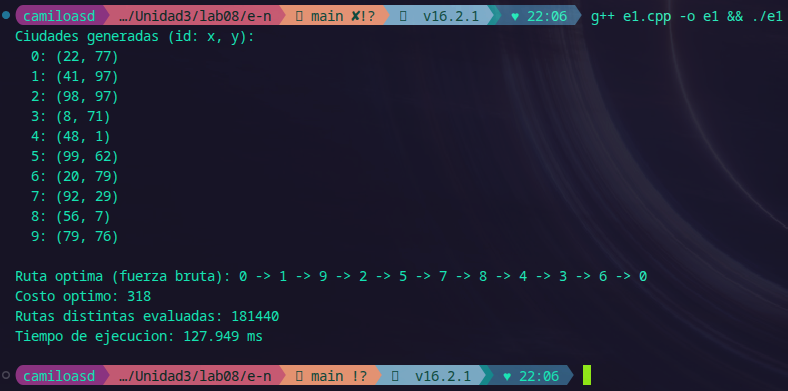
\includegraphics[width=0.8\textwidth]{../img/e1.png}
    \caption{Ejecución del ejercicio 1}
    \label{fig:e1}
\end{figure}

\subsection{Ejercicio 2}
Implementa búsqueda aleatoria (Monte Carlo) para el mismo TSP de 10 ciudades del ejercicio anterior, con distintos números de iteraciones (100, 1 000, 10 000), y compara qué tan cerca queda del óptimo real en cada caso.
\inputminted{cpp}{../e-n/e2.cpp}

\begin{itemize}
    \item /relleno
\end{itemize}

\begin{figure}[H]
    \centering
    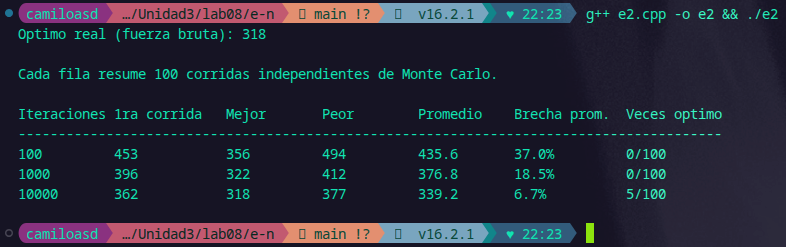
\includegraphics[width=0.8\textwidth]{../img/e2.png}
    \caption{Ejecución del ejercicio 2}
    \label{fig:e2}
\end{figure}

\subsection{Ejercicio 3}
Modela una versión simplificada del problema de programación de líneas de producción (por ejemplo, 6 tareas y 2 líneas) y resuélvela con búsqueda aleatoria, minimizando el tiempo total de finalización.
\inputminted{cpp}{../e-n/e3.cpp}

\begin{itemize}
    \item /relleno
\end{itemize}

\begin{figure}[H]
    \centering
    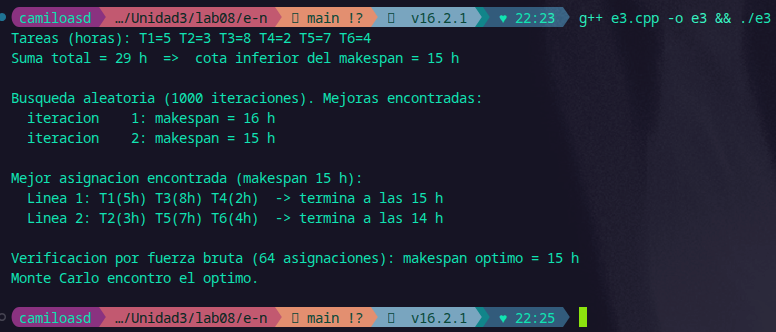
\includegraphics[width=0.8\textwidth]{../img/e3.png}
    \caption{Ejecución del ejercicio 3}
    \label{fig:e3}
\end{figure}

\subsection{Ejercicio 4}
Genera la gráfica de crecimiento del espacio de soluciones (como la Figura 3) para un problema de asignación de tareas (n! en vez de (n-1)!/2) y compárala con la del TSP.
\inputminted{cpp}{../e-n/e4.cpp}

\begin{itemize}
    \item /relleno
\end{itemize}

\begin{figure}[H]
    \centering
    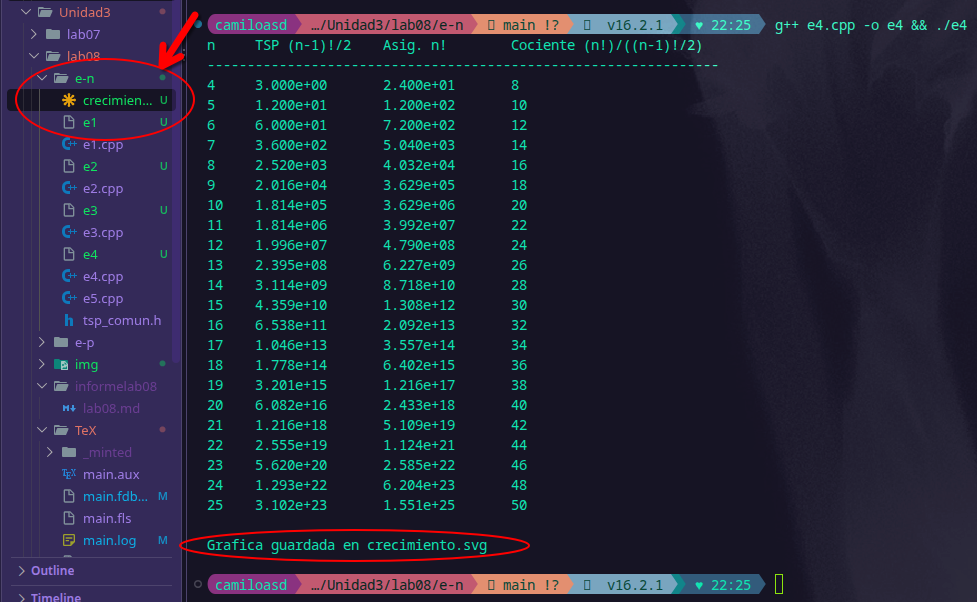
\includegraphics[width=0.8\textwidth]{../img/e4.png}
    \caption{Ejecución del ejercicio 4}
    \label{fig:e4}
\end{figure}

\subsection{Ejercicio 5}
Investiga y documenta un caso real donde se use el TSP o un problema de programación de líneas de producción (logística de reparto, planificación de manufactura, diseño de circuitos), indicando aproximadamente cuántas ciudades o tareas maneja en la práctica.
\inputminted{cpp}{../e-n/e5.cpp}

\begin{itemize}
    \item /relleno
\end{itemize}

\begin{figure}[H]
    \centering
    \includegraphics[width=0.8\textwidth]{../img/e5.png}
    \caption{Ejecución del ejercicio 5}
    \label{fig:e5}
\end{figure}

\section{Cuestionario}
\begin{itemize}
	\item ¿Cuál es la diferencia entre un problema de clase P y uno de clase NP?
	\item ¿Por qué se dice que el TSP es un problema NP-difícil?
	\item ¿Qué ventaja y qué desventaja principal tiene la búsqueda aleatoria (Monte Carlo) frente a la fuerza bruta?
	\item Si se aumenta el número de iteraciones de Monte Carlo, ¿qué se puede afirmar y qué NO se puede afirmar sobre la calidad de la solución encontrada?
	\item ¿Por qué la búsqueda aleatoria se considera solo un ``primer intento'' y no una solución definitiva para problemas NP-difíciles?
\end{itemize}

\section{Conclusiones}
% Pendiente de completar.

	%\begin{itemize}	
	%	\item Se creo el archivo \textbf{.gitignore} para no considerar los archivos %\textbf{*.class} que son innecesarios hacer seguimiento.
	%\end{itemize}
	%\begin{lstlisting}[language=bash]
	%	$ vim lab01/.gitignore
	%\end{lstlisting}
	%\begin{lstlisting}[language=bash]
	%	*.class
	%\end{lstlisting}
	%\begin{lstlisting}[language=bash]
	%	$ git add .
	%	$ git commit -m "Creando .gitignore para archivos *.class"			
	%	$ git push -u origin main
	%\end{lstlisting}
	
	%\begin{lstlisting}[language=bash]
	%	$ vim lab01/Insertion.java
	%\end{lstlisting}
	
    
%\clearpage
%\bibliographystyle{apalike}
%\bibliographystyle{IEEEtranN}
%\bibliography{bibliography}
			
\end{document}\noindent\textbf{Enunciado:}
